\documentclass[11pt]{article}
\usepackage[margin=1in]{geometry}
\usepackage{iftex}
\ifLuaTeX
  \usepackage{fontspec}
  \setmainfont{Arial}
\fi
\usepackage{graphicx}
\usepackage{booktabs}
\usepackage{hyperref}
\usepackage{amsmath}
\usepackage{caption}
\usepackage{float}

\title{AI for Cyber Security -- Home Exam Report}
\author{StudentID/Kandidatnr: 10}
\date{}

\begin{document}
\maketitle
\begin{center}
  
\includegraphics[width=0.45\textwidth]{../figures/Kristiania_logo_22_rod.jpg}
\end{center}
\tableofcontents
\newpage

\section{Overview}
This report summarizes the work for Q1--Q3 and includes methods, results, and mandatory reflections for all three questions.

\section{Q1 -- UNSW-NB15 (Regression for Normal Behavior)}
\subsection{Method}
I model normal behavior as a regression problem and flag large prediction errors as suspicious. The target is
\begin{equation}
  y = \log(1 + sbytes)
\end{equation}
The model is trained on a heuristic benign subset (normal connection states and non-extreme rates), using duration, packet-count, and categorical context features (\texttt{proto}, \texttt{service}, \texttt{state}).
I use \texttt{sbytes} as a proxy for session intensity because source-byte volume captures flow-level load behavior while remaining continuous and directly modelable. This is theoretically suitable for volumetric attacks (e.g., DoS), which are expected to disrupt the normal byte-volume relation, while low-and-slow attacks may remain close to that relation and therefore produce smaller residuals.
Consistent with MC104 Lecture 02 (page 3), I treat $y$ as the dependent variable and the traffic/context variables as independent variables used to explain normal intensity behavior.
The Q1 training split contains 175{,}341 rows and 36 raw attributes. The heuristic benign subset used for regression contains 166{,}202 rows. The model uses six predictors before one-hot encoding (three numeric and three categorical).

\textbf{Problem type.} I do not optimize for attack-label classification during training. I instead model expected normal intensity and detect structured residual deviations at inference time.

\textbf{Model requirements.} The model must capture non-linear relationships and feature interactions, remain robust to heavy-tailed/noisy network traffic, and deliver stable behavior without extensive tuning.

\textbf{Why Random Forest.} A Random Forest regressor fits these requirements for tabular traffic data. It captures non-linear dependencies, handles interactions across encoded categorical and numeric features, and is typically robust to outliers. I constrain tree depth to reduce overfitting to benign noise.
Random Forest is an ensemble-learning method that combines many decision trees (bagging) to reduce variance and improve robustness, consistent with MC104 L04 (Ensemble Learning).
This reflects a bias--variance trade-off. Limiting depth increases bias slightly but improves generalization stability by reducing variance.

\textbf{Trade-offs accepted.} I accept weaker extrapolation outside observed benign ranges and less direct interpretability than linear coefficients. The approach also assumes the benign subset is representative of normal traffic. The goal is not perfect regression accuracy, but stable normal-behavior modeling so attacks produce structured residual deviations.

An adaptive anomaly rule is then defined using the Median Absolute Deviation (MAD) of residuals, avoiding a fixed threshold.
As shown in MC104 Lecture 02 (pp. 17--19), the residual term $(Y_i-\hat{Y}_i)$ represents the unexplained component of the model. In this work, large structured residuals are interpreted as systematic deviations rather than random noise.
In practice, this means a flow is flagged when its error is unusually large relative to the benign error distribution, not because it crosses a fixed global cutoff.

\subsection{Results}
Figure~\ref{fig:q1-residual} shows residual differences by attack category. Figure~\ref{fig:q1-suspicious} shows the MAD-based suspicious rate. Figure~\ref{fig:q1-normal-vs-attack} compares normal vs attack median residuals.
In the aggregate Normal-vs-Attack summary, the attack median can appear lower because low-volume/low-and-slow attack categories dominate the count, while DoS-like categories still show larger deviations in the per-category view.
This highlights how aggregated statistics can be misleading when attack categories differ substantially in behavior.

\begin{figure}[H]
  \centering
  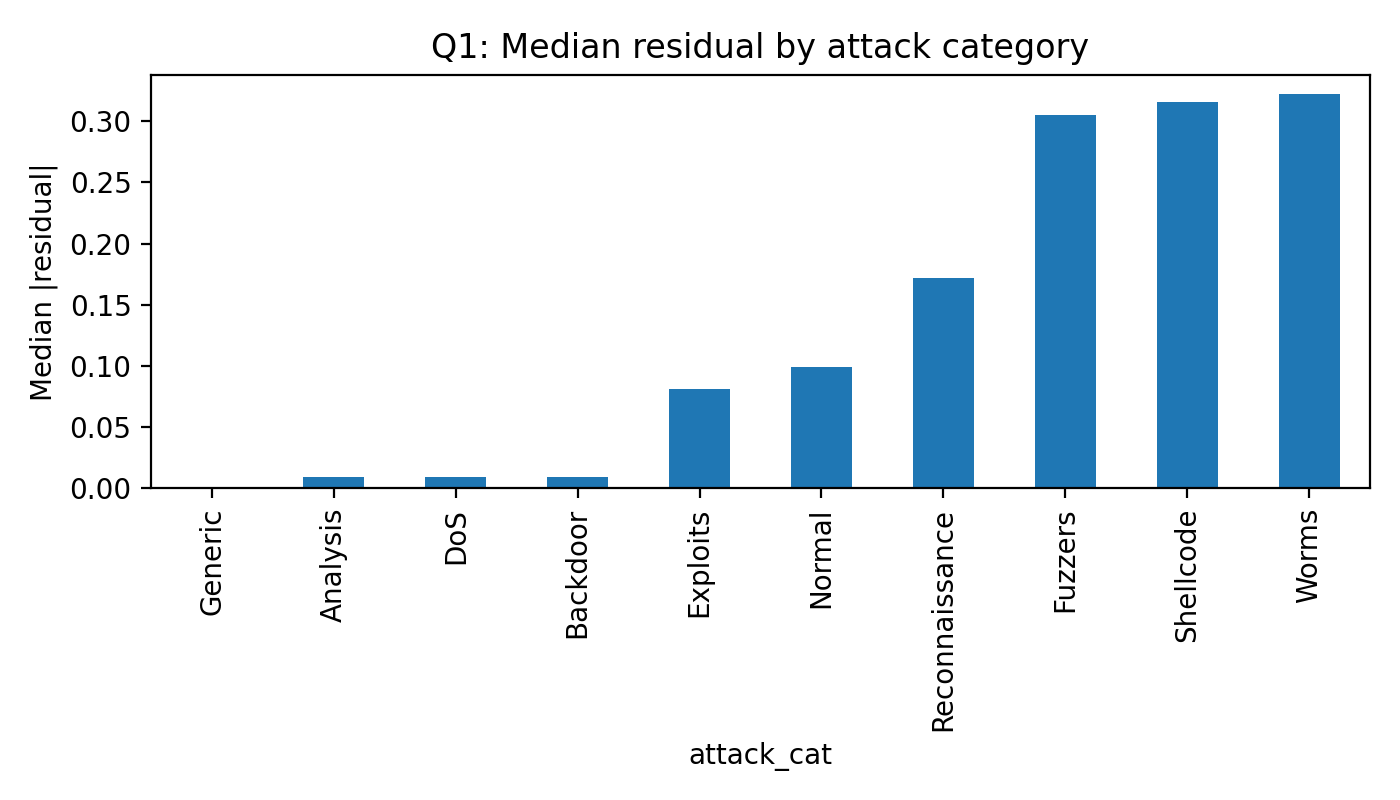
\includegraphics[width=0.8\textwidth]{../figures/q1_residual_median_by_attack.png}
  \caption{Median residual by attack category (Q1).}
  \label{fig:q1-residual}
\end{figure}
Key takeaway: volumetric categories tend to deviate more strongly, while low-volume categories remain closer to benign behavior.

\begin{figure}[H]
  \centering
  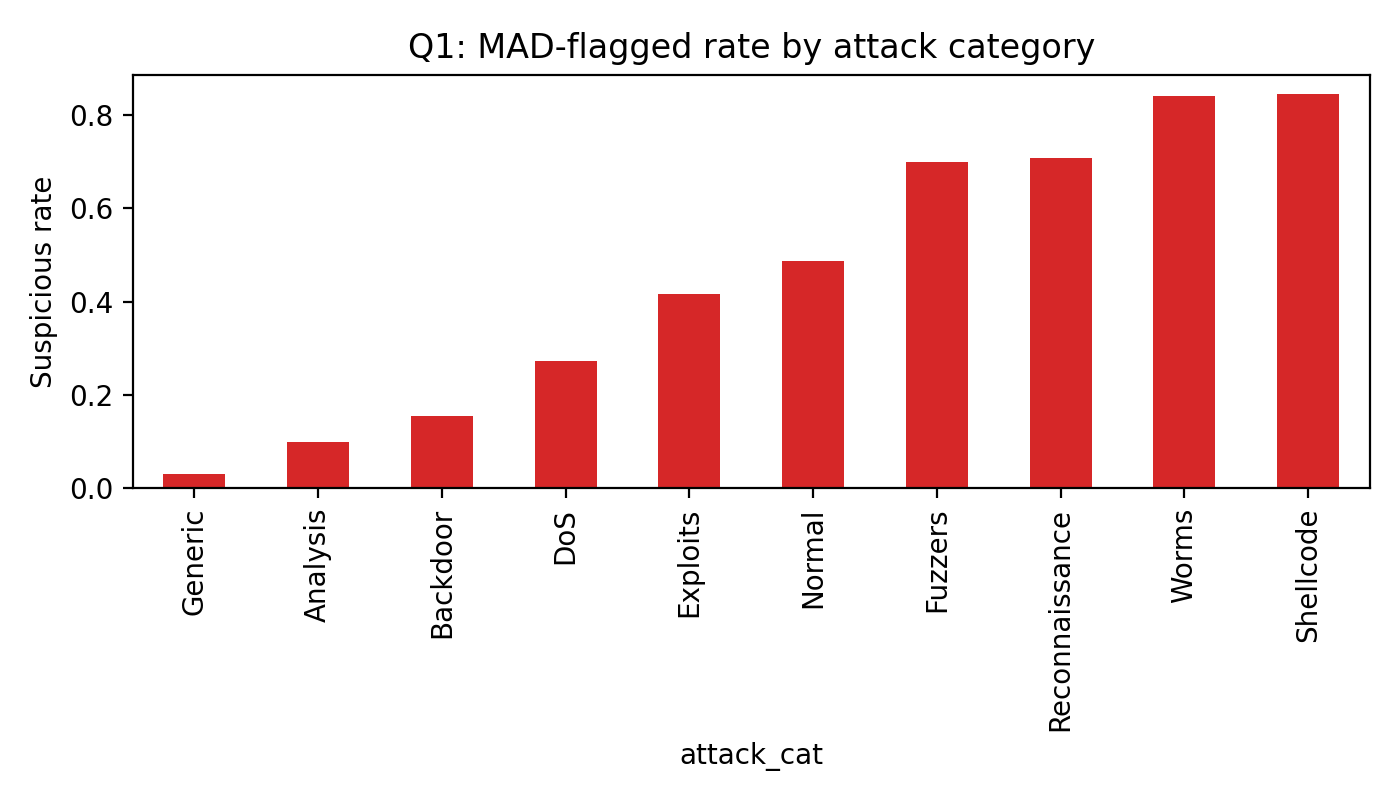
\includegraphics[width=0.8\textwidth]{../figures/q1_suspicious_rate_by_attack.png}
  \caption{MAD-flagged suspicious rate by attack category (Q1).}
  \label{fig:q1-suspicious}
\end{figure}

\begin{figure}[H]
  \centering
  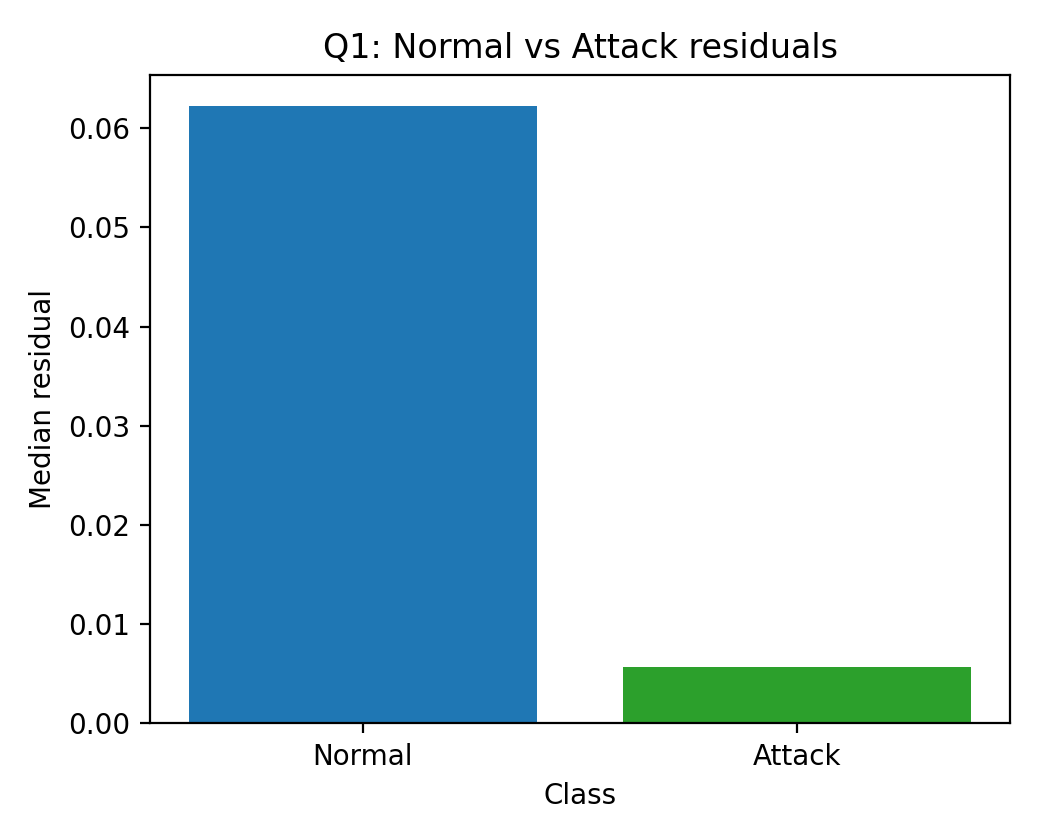
\includegraphics[width=0.6\textwidth]{../figures/q1_normal_vs_attack_median.png}
  \caption{Median residual for normal vs attack (Q1).}
  \label{fig:q1-normal-vs-attack}
\end{figure}

\subsection{Reflection}
\begin{itemize}
  \item \textbf{What did not work:} Low-and-slow and reconnaissance often yield small residuals, leading to false negatives.
  \item \textbf{Assumptions:} The method assumes normal traffic follows a stable relation between duration, packet counts, and byte volume. It also assumes the benign filter removes most attacks, and that byte volume is a useful proxy for abnormal behavior.
  \item Unlike classical unsupervised anomaly detection, this approach uses supervised regression on a filtered benign subset. It assumes attacks appear as structured residual deviations, not as arbitrary outliers.
  \item \textbf{Where it fails:} Concept drift (new services or traffic patterns) can invalidate the learned relation. Adaptive attackers can stay inside the normal error band. The model also cannot detect semantic or payload-level anomalies.
\end{itemize}

\section{Q2 -- NSL-KDD (Logistic Regression)}
\subsection{Method}
I build a binary classifier (attack vs normal) using logistic regression and explicitly test the linear-separability assumption. I start with five baseline features chosen from a security perspective: \texttt{duration} (persistence/session behavior), \texttt{src\_bytes} and \texttt{dst\_bytes} (traffic asymmetry and volumetric effects), \texttt{count} (repeated attempts in a time window), and \texttt{srv\_count} (bursting/scanning activity against services). Attack labels are mapped into categories (DoS, Probe, R2L, U2R) for error analysis.

I then modify the feature space without changing the model: logistic regression is kept fixed, while content/host features are added (\texttt{logged\_in}, \texttt{num\_failed\_logins}, \texttt{hot}, \texttt{num\_access\_files}, \texttt{dst\_host\_srv\_count}, \texttt{dst\_host\_same\_srv\_rate}) to test whether representation changes improve separability.
The Q2 training set contains 125{,}973 rows and 43 raw columns. I evaluate a 5-feature baseline and an 11-feature expanded representation while keeping the same logistic-regression model class.

Logistic regression assumes a global linear decision boundary in log-odds space, i.e., $\log\left(\frac{p}{1-p}\right)=w^T x$, which may be inappropriate for heterogeneous attack behaviors.
Following Ullah (MC104 Lecture 02, page 27), the linearity assumption is central to this evaluation. While logistic regression does not require normally distributed residuals as in OLS, it still depends on a globally linear relation in log-odds space and can fail when attack structure is heterogeneous.
Feature normalization was applied via \texttt{StandardScaler} to ensure comparable feature scales before linear modeling, consistent with lecture guidance on scaling and normalization (Ullah, MC104 Lecture 02, pp. 43--44).
As discussed in MC104 Logistic Regression Lecture 03, logistic regression imposes a global linear decision boundary in feature space through the log-odds formulation.

\subsection{Results}
Baseline accuracy is 66.3\%. The model works reasonably for DoS and Probe classes, which produce larger traffic-pattern deviations and are therefore closer to linearly separable in the baseline volume-based feature space. In contrast, the weakest categories are U2R and R2L (near-zero recall), indicating where linear separability breaks down.

These categories are low-volume and behavior/content-driven. They do not shift the initial feature space enough to form a clean linear boundary. After adding content/host features (without changing the model class), accuracy improves to 69.8\%, and recall improves for both U2R and R2L, showing that feature representation directly affects practical separability. Figure~\ref{fig:q2-recall} summarizes recall by category before and after feature expansion.

Empirically, DoS and Probe are approximately linearly separable in the chosen feature space, while U2R and R2L are not.
As discussed in MC104 L07 (Quantitative Metrics), aggregate accuracy can mask minority-class failure, which is consistent with the near-zero recall observed for U2R and R2L in the baseline setup.
Figure~\ref{fig:q2-recall} compares recall under the 5-feature baseline and the 11-feature representation that includes additional content and host variables.

\begin{figure}[H]
  \centering
  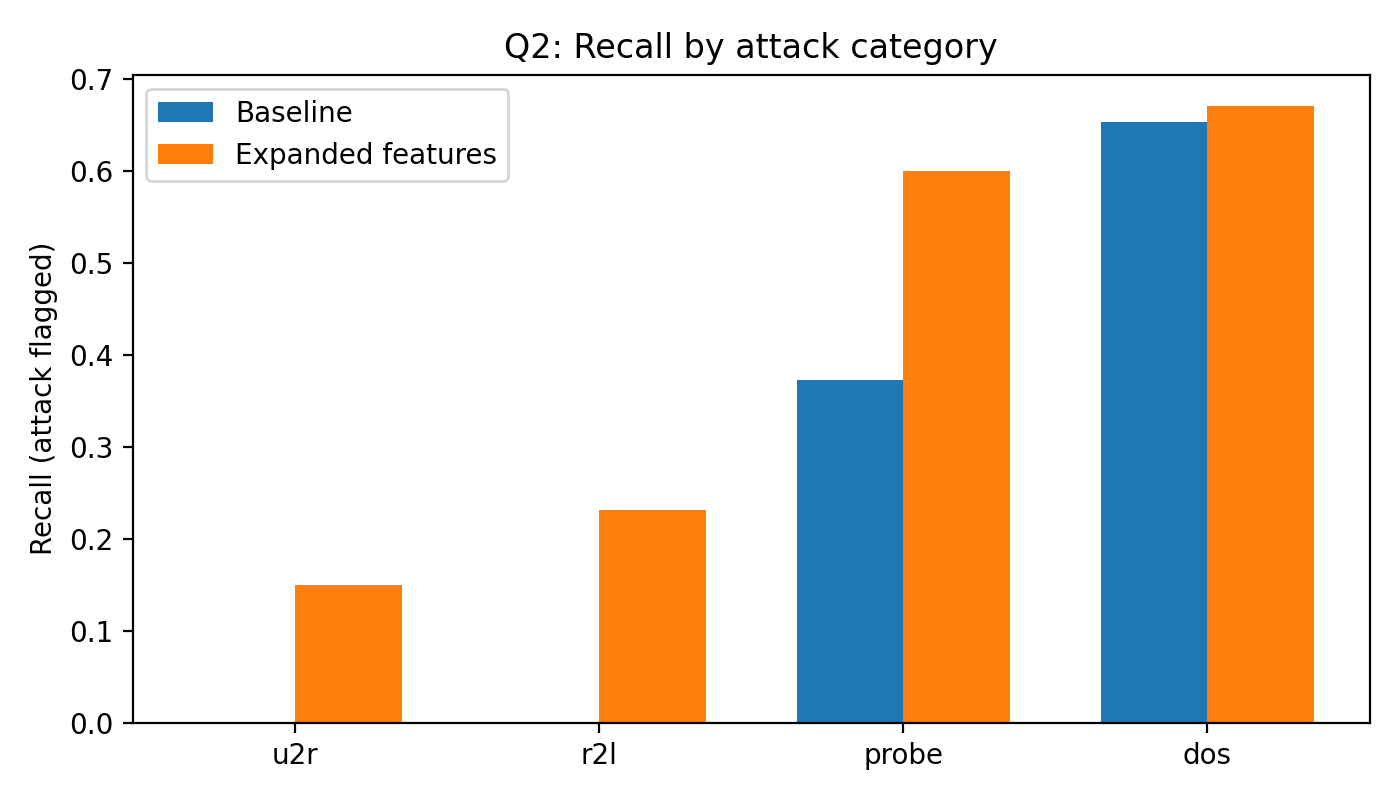
\includegraphics[width=0.8\textwidth]{../figures/q2_recall_by_attack_baseline_vs_v2.png}
  \caption{Recall by attack category (baseline vs expanded features, Q2).}
  \label{fig:q2-recall}
\end{figure}
Key takeaway: feature expansion mainly improves weak categories (U2R/R2L), showing that representation changes separability even when the model is unchanged.

\subsection{Reflection}
\begin{itemize}
  \item \textbf{What did not work:} The baseline feature space collapsed on minority categories (especially U2R and R2L), even when overall metrics looked acceptable.
  \item \textbf{Should I trust a model that performs well but violates assumptions?} Only partially. High aggregate accuracy can hide severe minority-class failure when true class structure is not linearly separable.
  \item This demonstrates that good performance under violated assumptions may reflect dataset bias rather than true model validity.
  \item \textbf{Is interpretability always an advantage?} Not necessarily. A linear boundary is easy to inspect, but interpretability does not guarantee correctness under heterogeneous attack behavior.
  \item \textbf{Deployment implication:} As traffic and attacker behavior drift, the feature space and model must be revalidated. Otherwise, linear assumptions will silently degrade detection quality.
  \item Across Q1 and Q2, one recurring theme is that representation strongly influences what appears detectable. In Q1, detection depends on stable residual structure, while in Q2, separability depends on feature expressiveness.
\end{itemize}

\section{Q3 -- Malimg (CNN)}
\subsection{Method}
I train a small CNN from scratch on Malimg (no pre-trained cyber models). The baseline uses standard cross-entropy. To address class imbalance, I compare it against a class-weighted loss. I evaluate accuracy and balanced accuracy, and I test robustness using a simple blur perturbation to probe whether the model relies on superficial texture artifacts.
The architecture is intentionally moderate in size, with three convolutional blocks (Conv-ReLU-MaxPool, 32/64/128 channels), followed by a dense layer (256 units), dropout (0.3), and final classification. It is large enough to learn discriminative patterns, but small enough to reduce overfitting to narrow texture artifacts.
The model is optimized with Adam and cross-entropy loss, consistent with MC104 L05 (MLP) and MC104 L08 (DL Optimizers).
The Malimg split used here contains 7{,}459 training images, 923 validation images, and 957 test images across 25 malware families, resized to 128$\times$128 inputs.

\subsection{Results}
Baseline test accuracy is 97.9\%, with balanced accuracy 93.9\%. Class-weighted test accuracy is 97.8\%, with balanced accuracy 93.8\%. Under blur perturbation, baseline accuracy drops to 72.1\% (balanced: 74.7\%), while the class-weighted model drops to 77.1\% (balanced: 86.8\%), indicating sensitivity to visual artifacts.
From a deployment perspective, the blur test approximates realistic visual shifts such as obfuscation, compression artifacts, and rendering variation.

\begin{figure}[H]
  \centering
  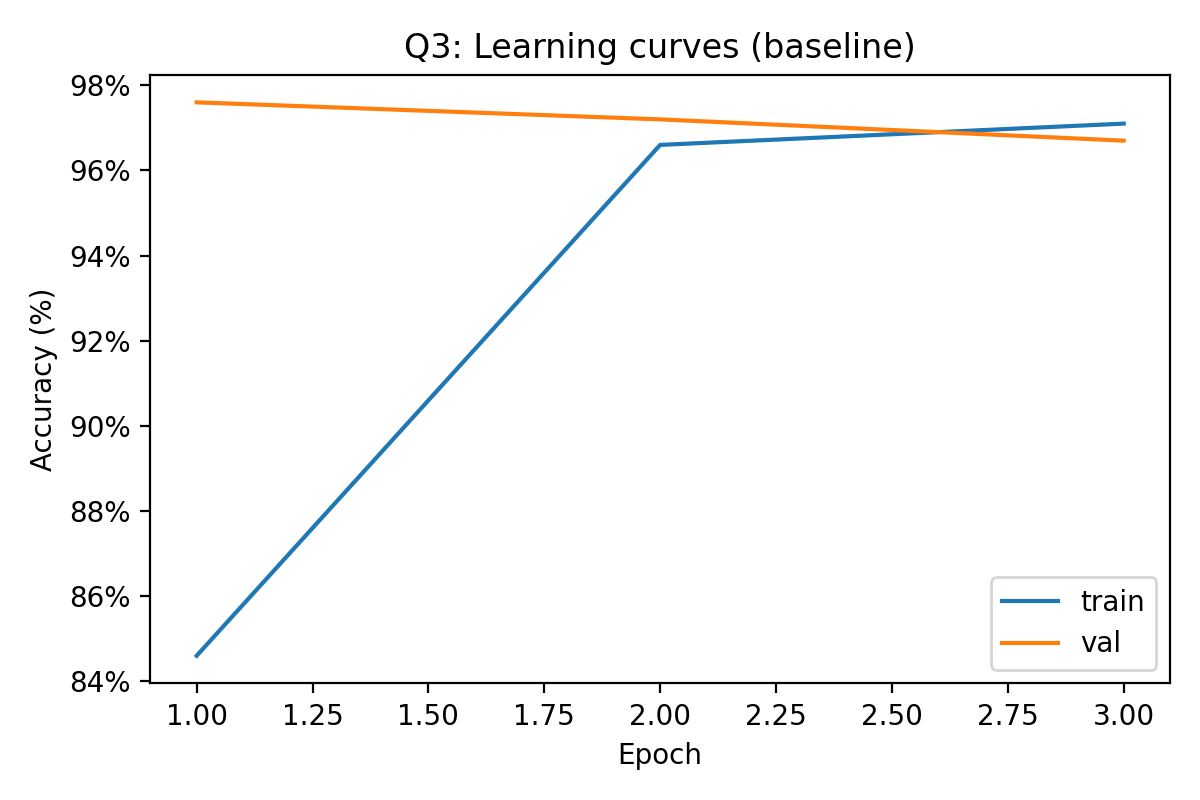
\includegraphics[width=0.7\textwidth]{../figures/q3_learning_curves_baseline.png}
  \caption{Learning curves for the baseline CNN (Q3).}
  \label{fig:q3-lc-base}
\end{figure}

\begin{figure}[H]
  \centering
  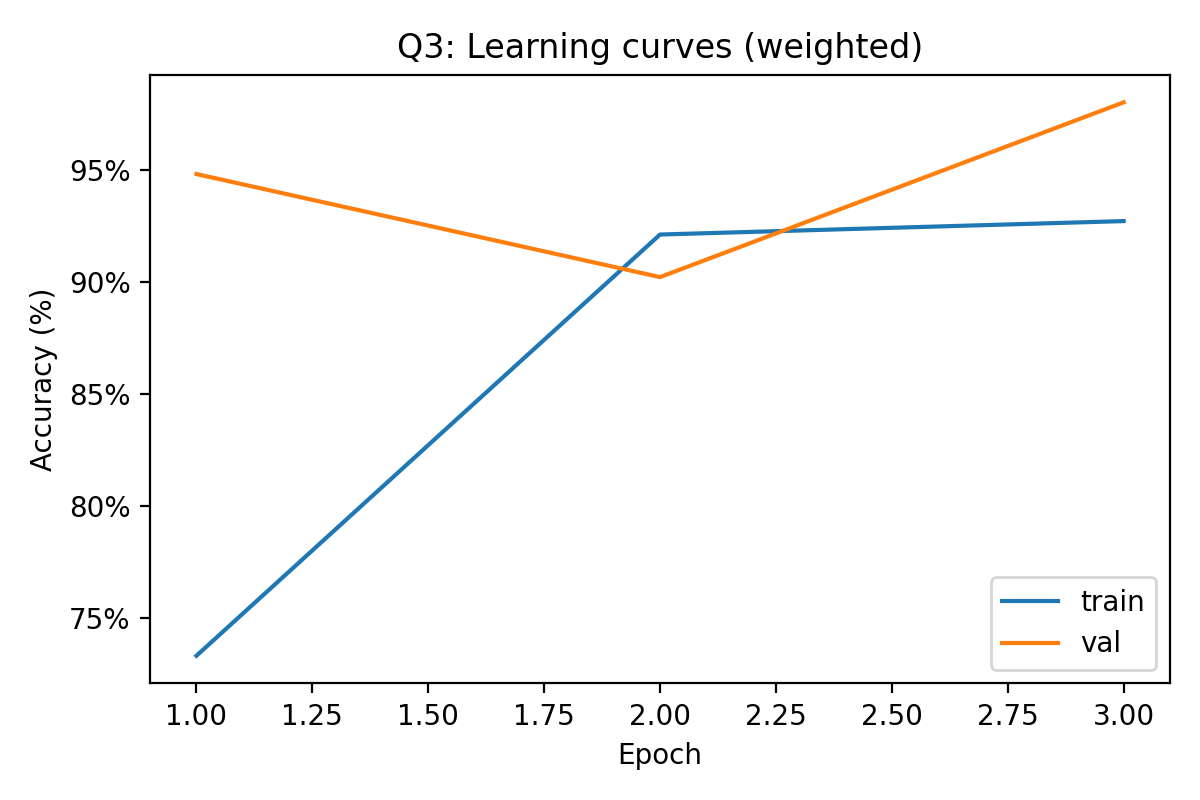
\includegraphics[width=0.7\textwidth]{../figures/q3_learning_curves_weighted.png}
  \caption{Learning curves for the class-weighted CNN (Q3).}
  \label{fig:q3-lc-weighted}
\end{figure}

\IfFileExists{../figures/q3_confusion_matrix_baseline_annot.png}{%
\begin{figure}[H]
  \centering
  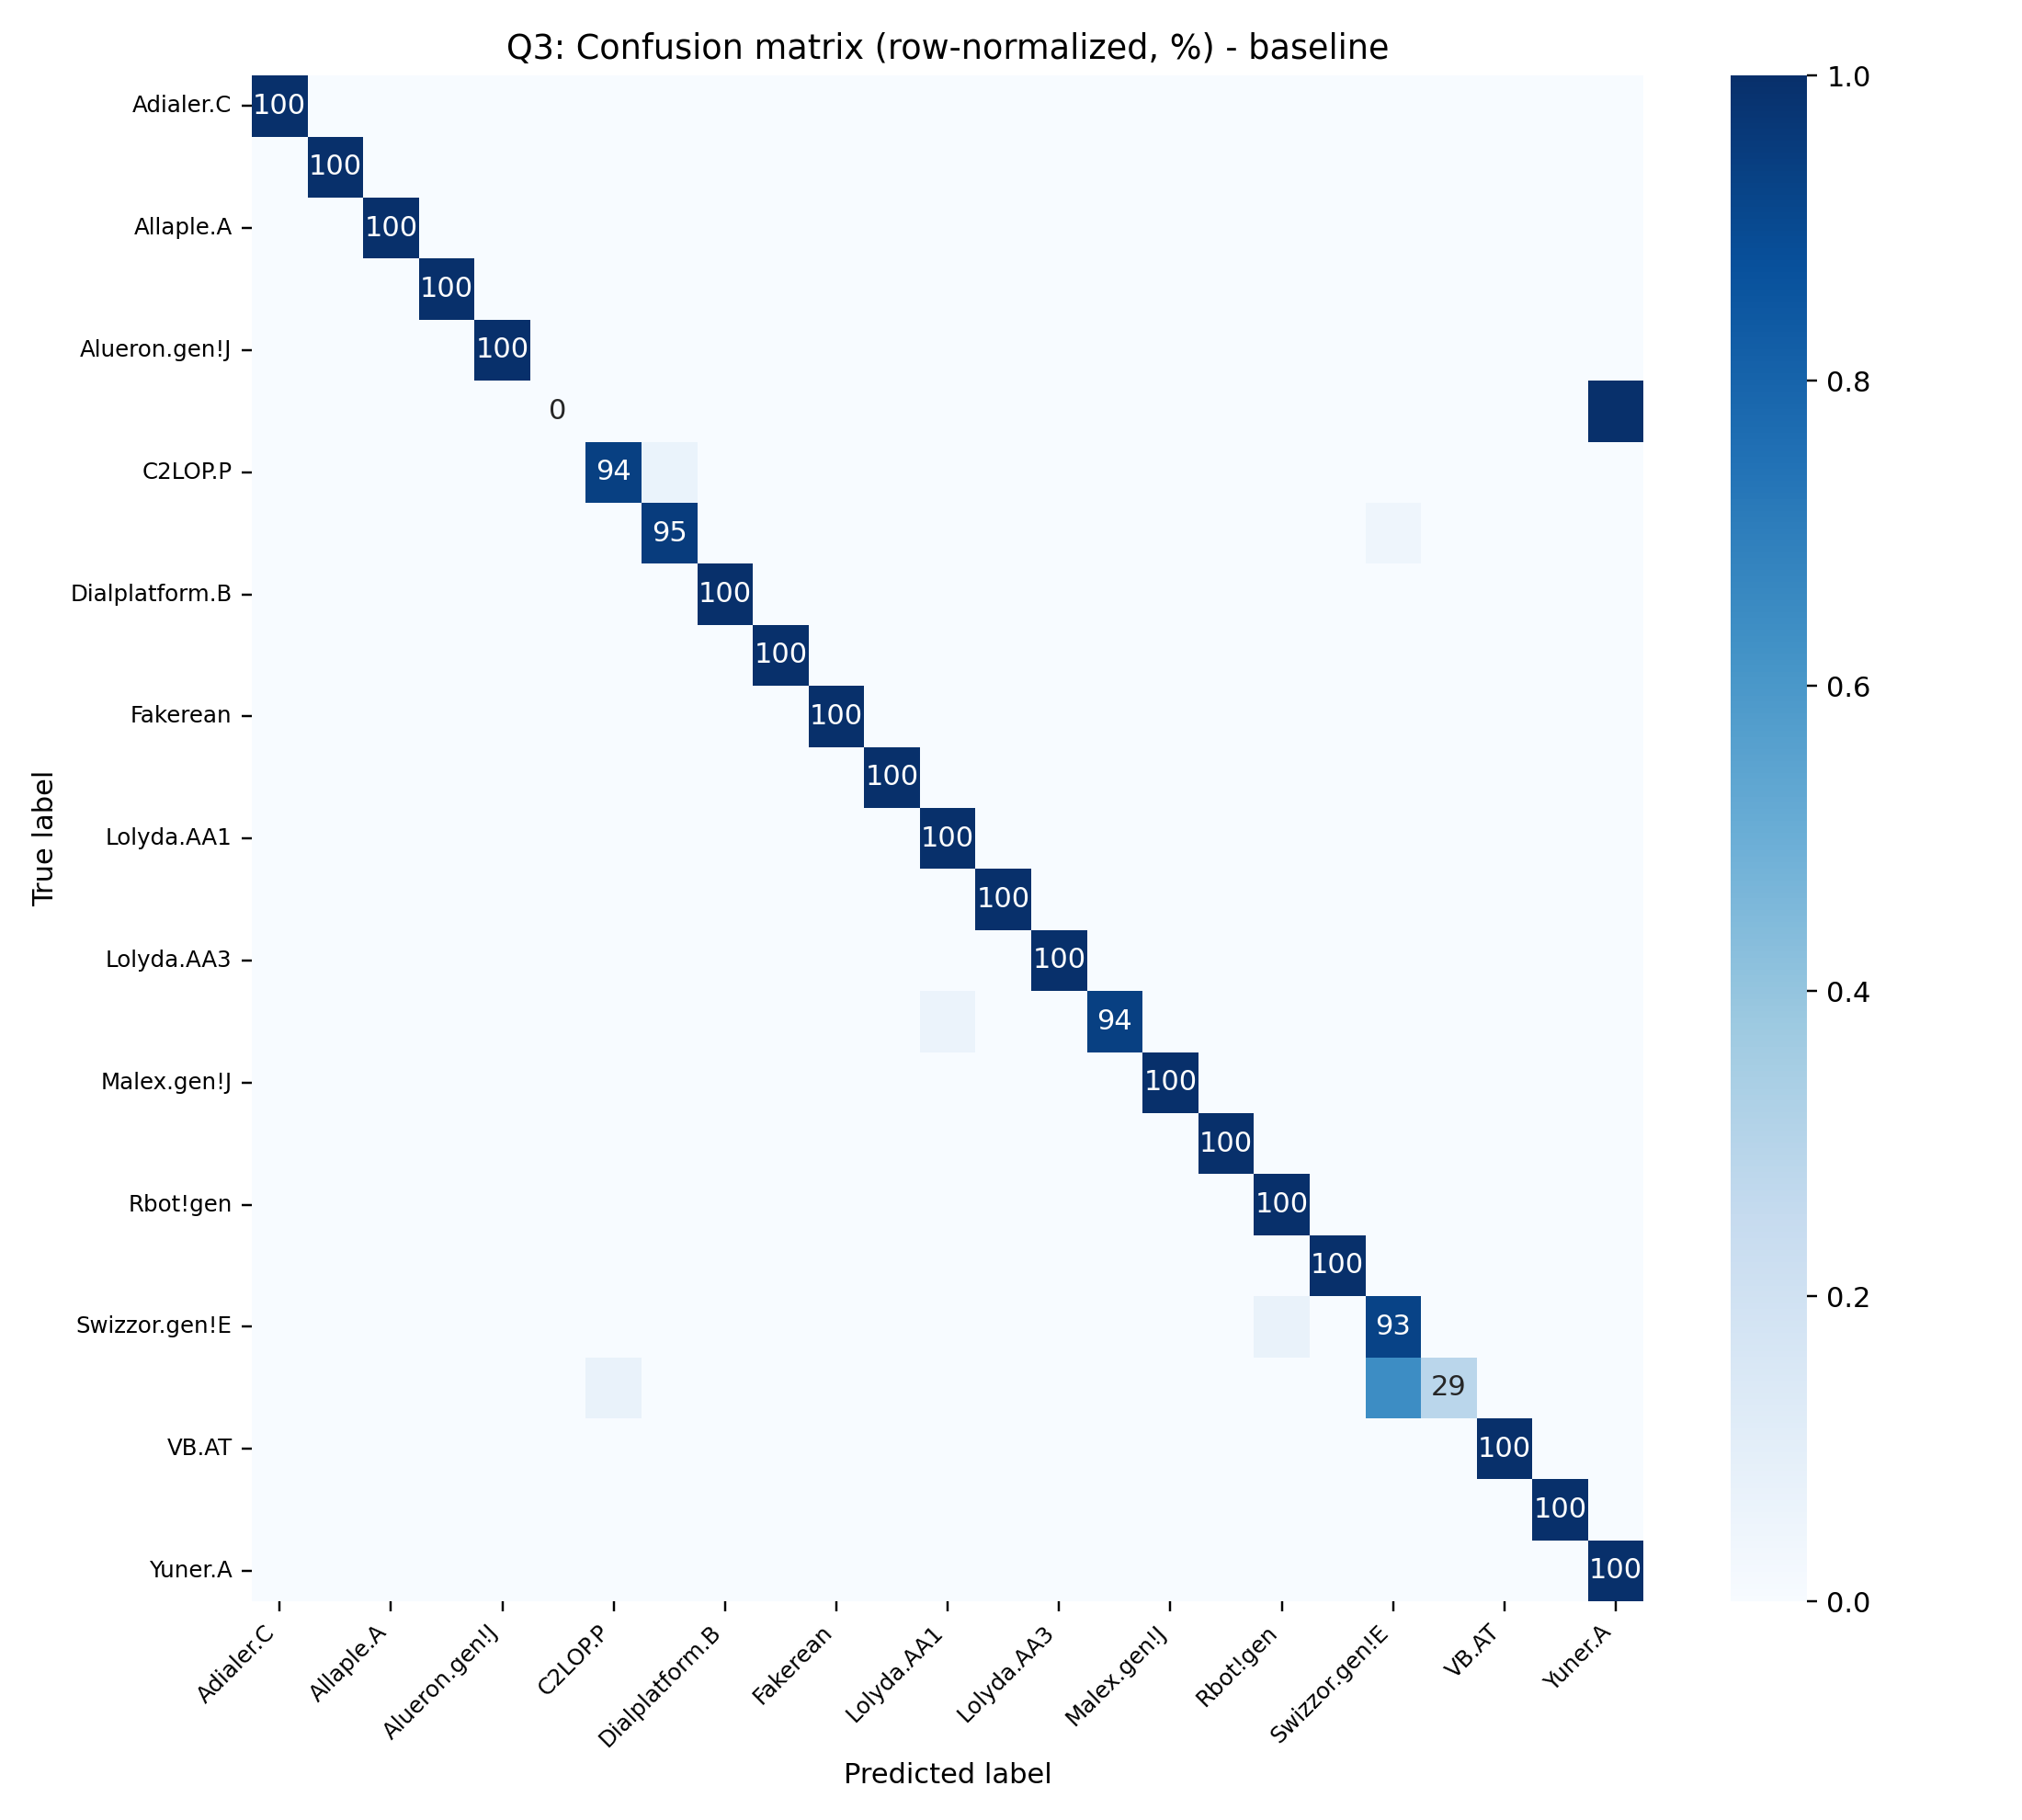
\includegraphics[width=0.95\textwidth]{../figures/q3_confusion_matrix_baseline_annot.png}
  \caption{Row-normalized confusion matrix (\%) for baseline CNN (Q3).}
  \label{fig:q3-cm-base}
\end{figure}
}{}

\IfFileExists{../figures/q3_confusion_matrix_weighted_annot.png}{%
\begin{figure}[H]
  \centering
  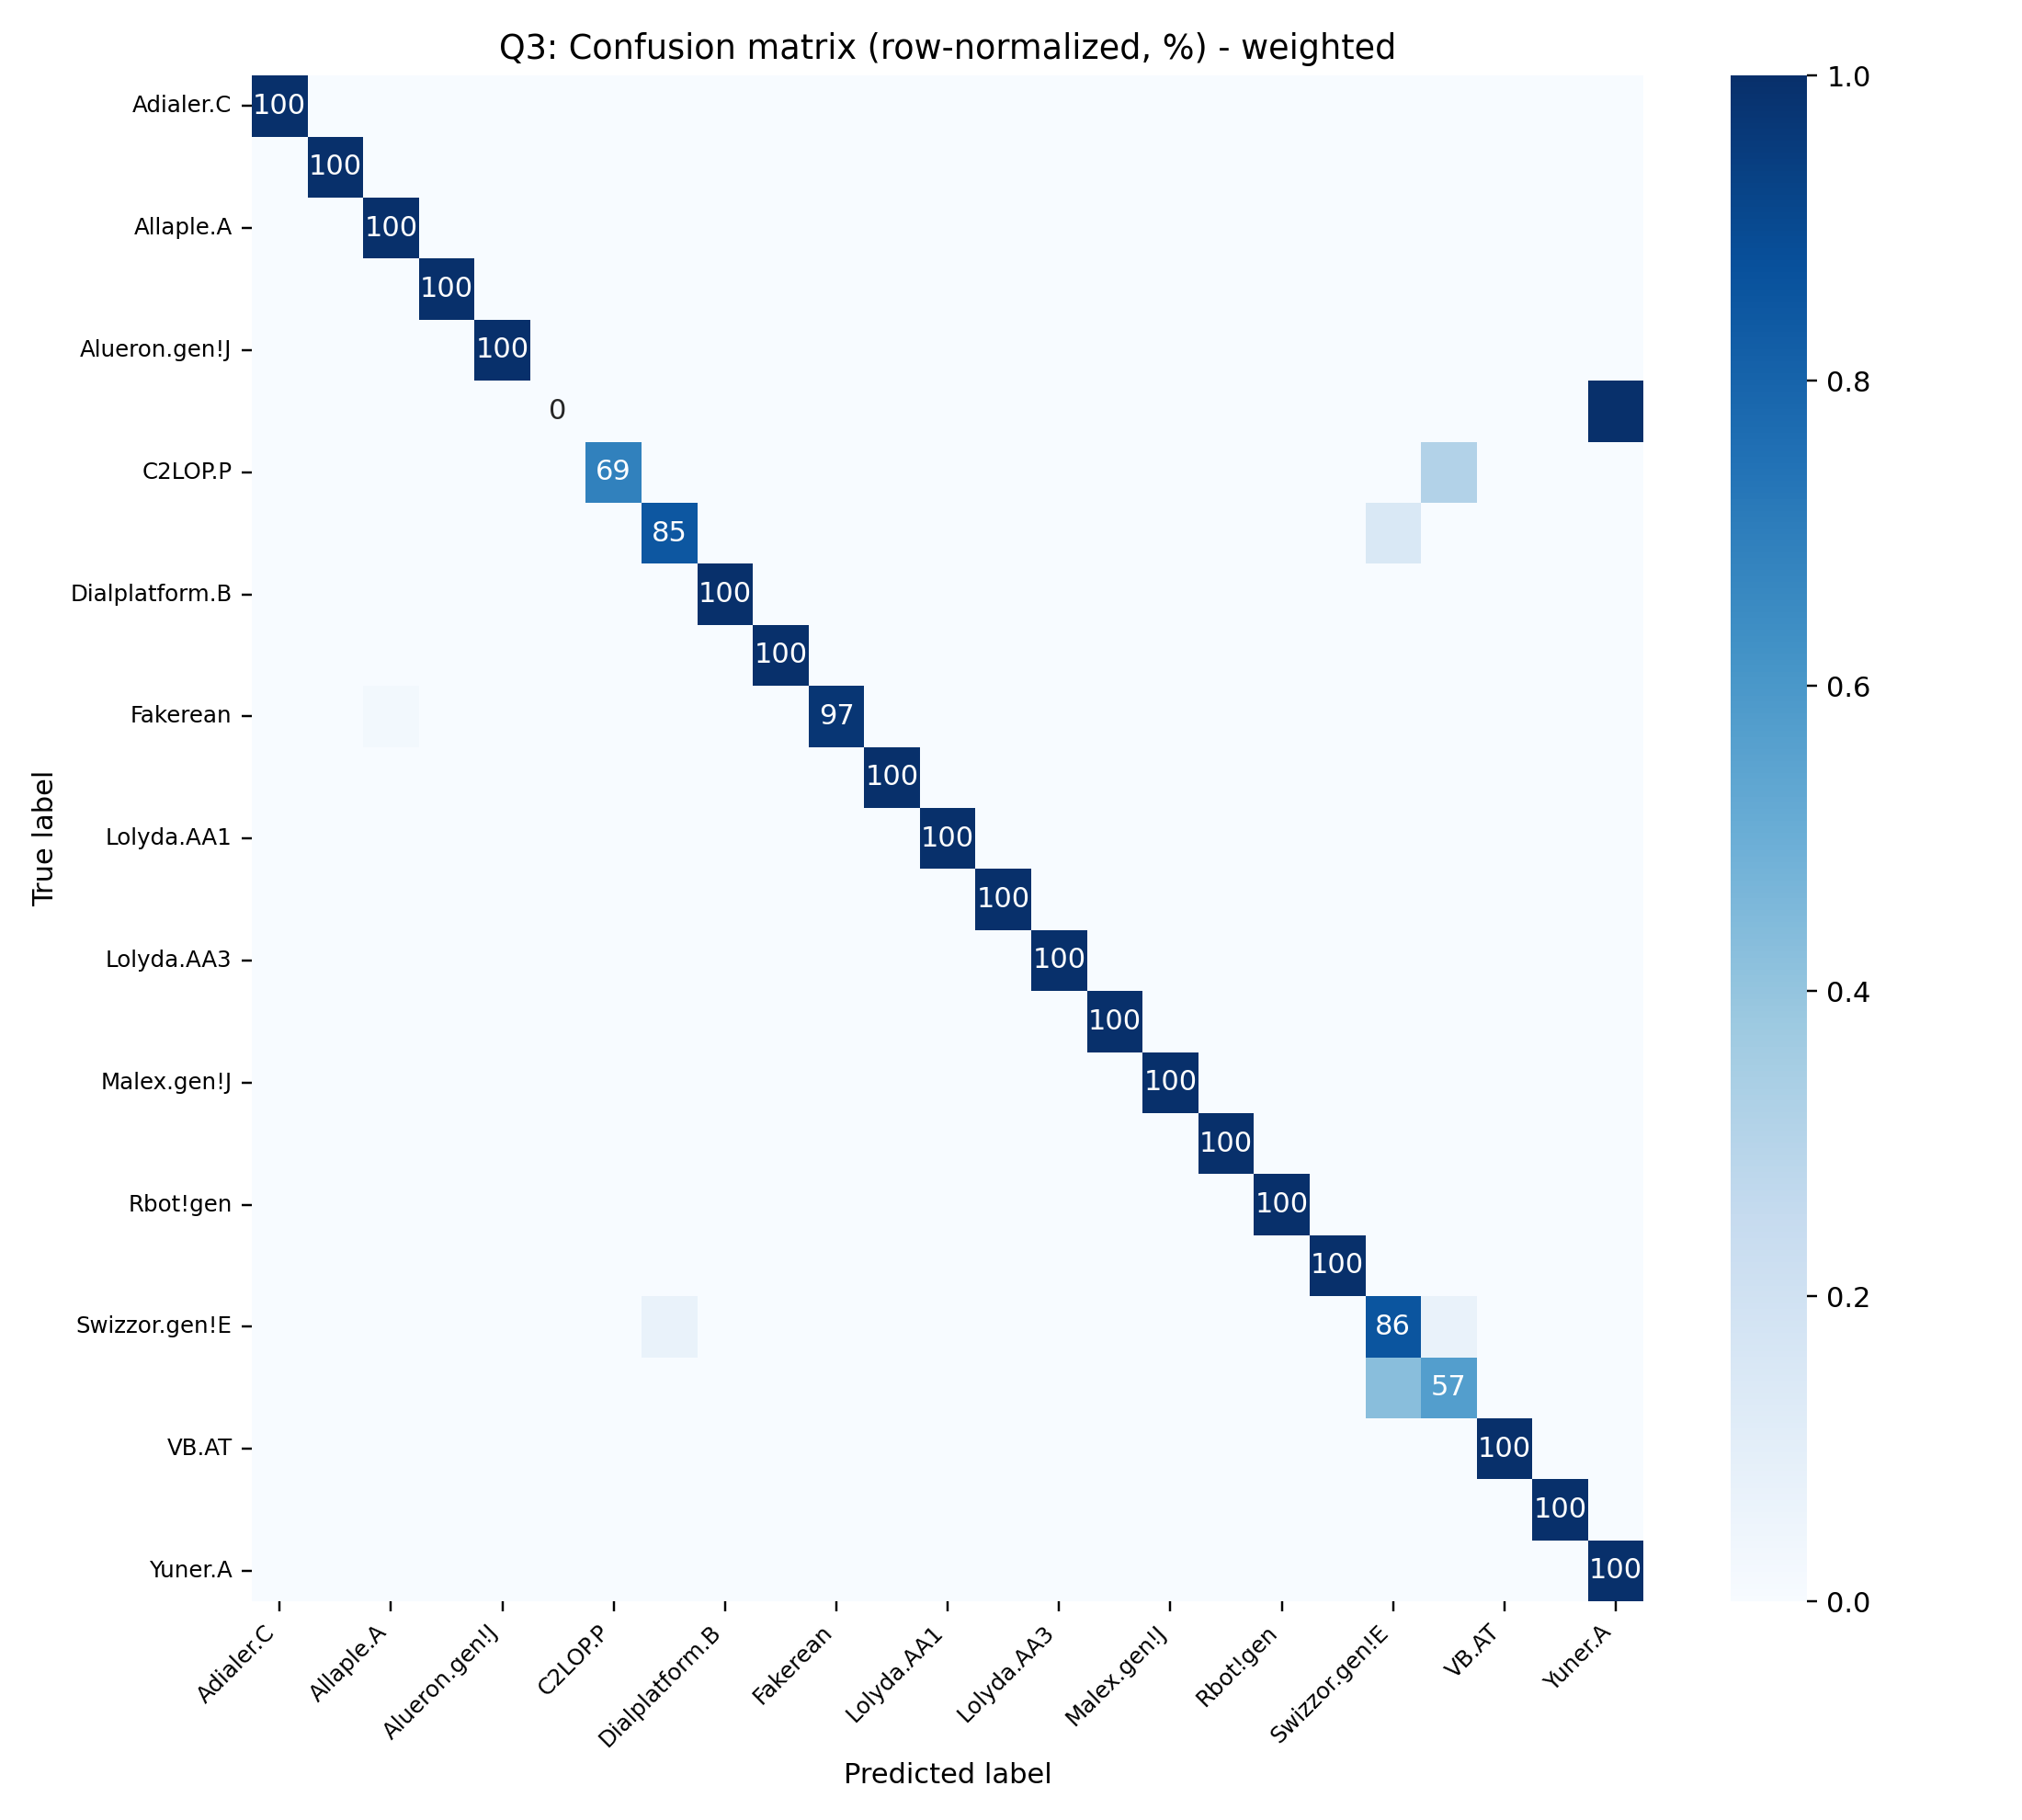
\includegraphics[width=0.95\textwidth]{../figures/q3_confusion_matrix_weighted_annot.png}
  \caption{Row-normalized confusion matrix (\%) for class-weighted CNN (Q3).}
  \label{fig:q3-cm-weighted}
\end{figure}
}{}

Cells with values below 1\% are intentionally left unannotated to preserve readability and avoid visual clutter.

\subsection{What it learns}
The sharp accuracy drop under blur suggests the CNN relies on fine-grained, high-frequency texture and edge cues rather than stable malware structure. This implies that packing, obfuscation, or minor rendering changes could significantly degrade performance. The weighted model is slightly more robust under blur, but sensitivity remains, so I treat image-based detection as a fragile signal rather than a standalone detector. This aligns with MC104 L06 (Visual Features), where CNN feature learning is tied to local textures and edges, and with MC104 L08 (Adversarial Attacks), where small perturbations can disproportionately affect model predictions.

\subsection{Reflection}
\begin{itemize}
  \item Malware image classification can be fragile because visual artifacts are easy to change without altering malicious intent.
  \item I should not blindly trust high accuracy from opaque models. Robustness tests are essential.
  \item In a real system, I would add robustness training, monitor drift, and combine image-based signals with semantic features.
\end{itemize}

\section{Reproducibility}
All experiments were run in a local Python virtual environment. Figures are generated into the \texttt{figures/} directory and the report source lives in \texttt{reports/}.

\section{Libraries Used}
\textbf{Core packages:} Python 3.12, NumPy, Pandas, SciPy, scikit-learn, Matplotlib, Seaborn.

\textbf{Deep learning stack:} PyTorch, torchvision, torchmetrics.

\textbf{Utilities:} Jupyter Notebook.

\section{References}
\begin{itemize}
  \item UNSW-NB15 dataset (Q1): \url{https://www.kaggle.com/datasets/dhoogla/unswnb15}
  \item NSL-KDD dataset (Q2): \url{https://www.kaggle.com/datasets/hassan06/nslkdd}
  \item Malimg dataset (Q3): \url{https://www.kaggle.com/datasets/manmandes/malimg}
  \item Ullah, Mohib. \textit{MC104\_Lecture02\_Regression.pdf}, Kristiania (Canvas course material, 2026), pages 3, 17--19, 27, 43--44.
  \item Ullah, Mohib. \textit{MC104-L04-EnsembleLearning-27Jan.pptx}, Kristiania (Canvas course material, 2026).
  \item Ullah, Mohib. \textit{MC104\_LogisticRegression\_Lecture03.pdf}, Kristiania (Canvas course material, 2026).
  \item Ullah, Mohib. \textit{MC104-L07-QuantitativeMetrics.pptx}, Kristiania (Canvas course material, 2026).
  \item Ullah, Mohib. \textit{MC104-L05-MLP-28Jan.pptx}, Kristiania (Canvas course material, 2026).
  \item Ullah, Mohib. \textit{MC104-L06-VisualFeatures-29Jan.pptx}, Kristiania (Canvas course material, 2026).
  \item Ullah, Mohib. \textit{MC104-L08-AdversarialAttacks.pdf}, Kristiania (Canvas course material, 2026).
  \item Ullah, Mohib. \textit{MC104-L08-DLOptimizers.pdf}, Kristiania (Canvas course material, 2026), p. 38--39, 45.
\end{itemize}

\end{document}
